\documentclass[ucs, notheorems, handout]{beamer}

\usetheme[numbers,totalnumbers,compress, nologo]{Statmod}
\usefonttheme[onlymath]{serif}
\setbeamertemplate{navigation symbols}{}

%\mode<handout> {
%    \usepackage{pgfpages}
%    \setbeameroption{show notes}
%    \pgfpagesuselayout{2 on 1}[a4paper, border shrink=5mm]
%    \setbeamercolor{note page}{bg=white}
%    \setbeamercolor{note title}{bg=gray!10}
%    \setbeamercolor{note date}{fg=gray!10}
%}

\usepackage[utf8x]{inputenc}
\usepackage[T2A]{fontenc}
\usepackage[english, russian]{babel}
\usepackage{tikz}
\usepackage{ragged2e}
\usepackage{wrapfig}
\usepackage{t-angles}
\usepackage{slashbox}
\usepackage{hhline}
\usepackage{multirow}
\usepackage{graphics}
%new calligraphic font for subspaces 
\usepackage{euscript}
\newcommand{\cA}{\EuScript{A}}
\newcommand{\cB}{\EuScript{B}}
\newcommand{\cC}{\EuScript{C}}
\newcommand{\cD}{\EuScript{D}}
\newcommand{\cE}{\EuScript{E}}
\newcommand{\cF}{\EuScript{F}}
\newcommand{\cG}{\EuScript{G}}
\newcommand{\cH}{\EuScript{H}}
\newcommand{\cI}{\EuScript{I}}
\newcommand{\cJ}{\EuScript{J}}
\newcommand{\cK}{\EuScript{K}}
\newcommand{\cL}{\EuScript{L}}
\newcommand{\cM}{\EuScript{M}}
\newcommand{\cN}{\EuScript{N}}
\newcommand{\cO}{\EuScript{O}}
\newcommand{\cP}{\EuScript{P}}
\newcommand{\cQ}{\EuScript{Q}}
\newcommand{\cR}{\EuScript{R}}
\newcommand{\cS}{\EuScript{S}}
\newcommand{\cT}{\EuScript{T}}
\newcommand{\cU}{\EuScript{U}}
\newcommand{\cV}{\EuScript{V}}
\newcommand{\cW}{\EuScript{W}}
\newcommand{\cX}{\EuScript{X}}
\newcommand{\cY}{\EuScript{Y}}
\newcommand{\cZ}{\EuScript{Z}}

%font for text indices like transposition X^\mathrm{T}
\newcommand{\rmA}{\mathrm{A}}
\newcommand{\rmB}{\mathrm{B}}
\newcommand{\rmC}{\mathrm{C}}
\newcommand{\rmD}{\mathrm{D}}
\newcommand{\rmE}{\mathrm{E}}
\newcommand{\rmF}{\mathrm{F}}
\newcommand{\rmG}{\mathrm{G}}
\newcommand{\rmH}{\mathrm{H}}
\newcommand{\rmI}{\mathrm{I}}
\newcommand{\rmJ}{\mathrm{J}}
\newcommand{\rmK}{\mathrm{K}}
\newcommand{\rmL}{\mathrm{L}}
\newcommand{\rmM}{\mathrm{M}}
\newcommand{\rmN}{\mathrm{N}}
\newcommand{\rmO}{\mathrm{O}}
\newcommand{\rmP}{\mathrm{P}}
\newcommand{\rmQ}{\mathrm{Q}}
\newcommand{\rmR}{\mathrm{R}}
\newcommand{\rmS}{\mathrm{S}}
\newcommand{\rmT}{\mathrm{T}}
\newcommand{\rmU}{\mathrm{U}}
\newcommand{\rmV}{\mathrm{V}}
\newcommand{\rmW}{\mathrm{W}}
\newcommand{\rmX}{\mathrm{X}}
\newcommand{\rmY}{\mathrm{Y}}
\newcommand{\rmZ}{\mathrm{Z}}

%tt font for time series
\newcommand{\tA}{\mathsf{A}}
\newcommand{\tB}{\mathsf{B}}
\newcommand{\tC}{\mathsf{C}}
\newcommand{\tD}{\mathsf{D}}
\newcommand{\tE}{\mathsf{E}}
\newcommand{\tF}{\mathsf{F}}
\newcommand{\tG}{\mathsf{G}}
\newcommand{\tH}{\mathsf{H}}
\newcommand{\tI}{\mathsf{I}}
\newcommand{\tJ}{\mathsf{J}}
\newcommand{\tK}{\mathsf{K}}
\newcommand{\tL}{\mathsf{L}}
\newcommand{\tM}{\mathsf{M}}
\newcommand{\tN}{\mathsf{N}}
\newcommand{\tO}{\mathsf{O}}
\newcommand{\tP}{\mathsf{P}}
\newcommand{\tQ}{\mathsf{Q}}
\newcommand{\tR}{\mathsf{R}}
\newcommand{\tS}{\mathsf{S}}
\newcommand{\tT}{\mathsf{T}}
\newcommand{\tU}{\mathsf{U}}
\newcommand{\tV}{\mathsf{V}}
\newcommand{\tW}{\mathsf{W}}
\newcommand{\tX}{\mathsf{X}}
\newcommand{\tY}{\mathsf{Y}}
\newcommand{\tZ}{\mathsf{Z}}

%bf font for matrices
\newcommand{\bfA}{\mathbf{A}}
\newcommand{\bfB}{\mathbf{B}}
\newcommand{\bfC}{\mathbf{C}}
\newcommand{\bfD}{\mathbf{D}}
\newcommand{\bfE}{\mathbf{E}}
\newcommand{\bfF}{\mathbf{F}}
\newcommand{\bfG}{\mathbf{G}}
\newcommand{\bfH}{\mathbf{H}}
\newcommand{\bfI}{\mathbf{I}}
\newcommand{\bfJ}{\mathbf{J}}
\newcommand{\bfK}{\mathbf{K}}
\newcommand{\bfL}{\mathbf{L}}
\newcommand{\bfM}{\mathbf{M}}
\newcommand{\bfN}{\mathbf{N}}
\newcommand{\bfO}{\mathbf{O}}
\newcommand{\bfP}{\mathbf{P}}
\newcommand{\bfQ}{\mathbf{Q}}
\newcommand{\bfR}{\mathbf{R}}
\newcommand{\bfS}{\mathbf{S}}
\newcommand{\bfT}{\mathbf{T}}
\newcommand{\bfU}{\mathbf{U}}
\newcommand{\bfV}{\mathbf{V}}
\newcommand{\bfW}{\mathbf{W}}
\newcommand{\bfX}{\mathbf{X}}
\newcommand{\bfY}{\mathbf{Y}}
\newcommand{\bfZ}{\mathbf{Z}}

%bb font for standard spaces and expectation
\newcommand{\bbA}{\mathbb{A}}
\newcommand{\bbB}{\mathbb{B}}
\newcommand{\bbC}{\mathbb{C}}
\newcommand{\bbD}{\mathbb{D}}
\newcommand{\bbE}{\mathbb{E}}
\newcommand{\bbF}{\mathbb{F}}
\newcommand{\bbG}{\mathbb{G}}
\newcommand{\bbH}{\mathbb{H}}
\newcommand{\bbI}{\mathbb{I}}
\newcommand{\bbJ}{\mathbb{J}}
\newcommand{\bbK}{\mathbb{K}}
\newcommand{\bbL}{\mathbb{L}}
\newcommand{\bbM}{\mathbb{M}}
\newcommand{\bbN}{\mathbb{N}}
\newcommand{\bbO}{\mathbb{O}}
\newcommand{\bbP}{\mathbb{P}}
\newcommand{\bbQ}{\mathbb{Q}}
\newcommand{\bbR}{\mathbb{R}}
\newcommand{\bbS}{\mathbb{S}}
\newcommand{\bbT}{\mathbb{T}}
\newcommand{\bbU}{\mathbb{U}}
\newcommand{\bbV}{\mathbb{V}}
\newcommand{\bbW}{\mathbb{W}}
\newcommand{\bbX}{\mathbb{X}}
\newcommand{\bbY}{\mathbb{Y}}
\newcommand{\bbZ}{\mathbb{Z}}

%got font for any case
\newcommand{\gA}{\mathfrak{A}}
\newcommand{\gB}{\mathfrak{B}}
\newcommand{\gC}{\mathfrak{C}}
\newcommand{\gD}{\mathfrak{D}}
\newcommand{\gE}{\mathfrak{E}}
\newcommand{\gF}{\mathfrak{F}}
\newcommand{\gG}{\mathfrak{G}}
\newcommand{\gH}{\mathfrak{H}}
\newcommand{\gI}{\mathfrak{I}}
\newcommand{\gJ}{\mathfrak{J}}
\newcommand{\gK}{\mathfrak{K}}
\newcommand{\gL}{\mathfrak{L}}
\newcommand{\gM}{\mathfrak{M}}
\newcommand{\gN}{\mathfrak{N}}
\newcommand{\gO}{\mathfrak{O}}
\newcommand{\gP}{\mathfrak{P}}
\newcommand{\gQ}{\mathfrak{Q}}
\newcommand{\gR}{\mathfrak{R}}
\newcommand{\gS}{\mathfrak{S}}
\newcommand{\gT}{\mathfrak{T}}
\newcommand{\gU}{\mathfrak{U}}
\newcommand{\gV}{\mathfrak{V}}
\newcommand{\gW}{\mathfrak{W}}
\newcommand{\gX}{\mathfrak{X}}
\newcommand{\gY}{\mathfrak{Y}}
\newcommand{\gZ}{\mathfrak{Z}}

%old calligraphic font
\newcommand{\calA}{\mathcal{A}}
\newcommand{\calB}{\mathcal{B}}
\newcommand{\calC}{\mathcal{C}}
\newcommand{\calD}{\mathcal{D}}
\newcommand{\calE}{\mathcal{E}}
\newcommand{\calF}{\mathcal{F}}
\newcommand{\calG}{\mathcal{G}}
\newcommand{\calH}{\mathcal{H}}
\newcommand{\calI}{\mathcal{I}}
\newcommand{\calJ}{\mathcal{J}}
\newcommand{\calK}{\mathcal{K}}
\newcommand{\calL}{\mathcal{L}}
\newcommand{\calM}{\mathcal{M}}
\newcommand{\calN}{\mathcal{N}}
\newcommand{\calO}{\mathcal{O}}
\newcommand{\calP}{\mathcal{P}}
\newcommand{\calQ}{\mathcal{Q}}
\newcommand{\calR}{\mathcal{R}}
\newcommand{\calS}{\mathcal{S}}
\newcommand{\calT}{\mathcal{T}}
\newcommand{\calU}{\mathcal{U}}
\newcommand{\calV}{\mathcal{V}}
\newcommand{\calW}{\mathcal{W}}
\newcommand{\calX}{\mathcal{X}}
\newcommand{\calY}{\mathcal{Y}}
\newcommand{\calZ}{\mathcal{Z}}


\setbeamercolor{bluetext_color}{fg=blue}
\newcommand{\bluetext}[1]{{\usebeamercolor[fg]{bluetext_color}#1}}

\newtheorem{theorem}{Теорема}
\newtheorem{statement}{Утверждение}

\title[Tensor SSA]{Тензорный анализ сингулярного спектра}

\author[Хромов Н.А., Голяндина Н.Э.]{\underline{Хромов Никита Андреевич}, Голяндина Нина Эдуардовна}

\institute[Санкт-Петербургский Государственный Университет]{%
    \small
    Санкт-Петербургский государственный университет\\
    Математико-механический факультет\\
    Кафедра статистического моделирования\\
    \vspace{1.25cm}
}

\date{Наука СПбГУ\\
    21 ноября 2023, Санкт-Петербург}

\subject{Talks}

\begin{document}

    \begin{frame}[plain]
        \titlepage

    \end{frame}


    \section{Введение}\label{sec:intro}
    \begin{frame}{Постановка задачи}
        Временной ряд длины $N$: $\tX=(x_1, x_2,\ldots, x_N)$, $x_i\in \mathbb{R}$.

        $\tX = \tS + \tP + \tR$.
        \vspace{0.8cm}

        \bluetext{Возможные задачи:}
        \begin{enumerate}
            \item Выделение сигнала из ряда: нахождение $\tT + \tP$;
            \item Отделение компонент сигнала: нахождение $\tT$ и $\tP$.
        \end{enumerate}

        \vspace{0.5cm}
        Одним из методов решения этих задач является метод Singular Spectrum Analysis
        (\bluetext{SSA}) \\(Golyandina et al. (2001), Analysis of time series structure: SSA and related techiques)

        \vspace{0.4cm}

        \textcolor{red}{Цель:} построение тензорных модификаций SSA для увеличения точности оценки сигнала.
    \end{frame}
    \begin{frame}{SSA для выделения сигнала}
        $\tX = (x_1, x_2, \dots, x_N) = \tS + \tR$,
        $L$ - длина окна, $K = N - L + 1 \geqslant L$.

        \vspace{0.3cm}

        \bluetext{Параметры алгоритма:} $L,\, R:\: R \leqslant L < N$.

        $R$ --- число компонент, отнесённых к сигналу.

        \vspace{0.3cm}

        \bluetext{Схема алгоритма SSA для выделения сигнала}
        \begin{enumerate}
            \item \bluetext{Вложение} $\tX \mapsto \bfX = [X_1, X_2, \dots, X_K]\in \bbR^{L\times K},$

            $X_i = (x_i, x_{i+1}, \dots, x_{i + L})^{\rmT}$

            \vspace{0.2cm}

            \item \bluetext{Разложение} $\bfX = \sum_{i=1}^{d} \sqrt{\lambda_i}U_i V_i^\rmT,\,\, d \leqslant L$

            \vspace{0.2cm}

            \item \bluetext{Группировка} $\tilde{\bfX}= \sum_{i=1}^{R} \sqrt{\lambda_i}U_i V_i^\rmT$

            \vspace{0.2cm}

            \item \bluetext{Восстановление} Матрица $\tilde{\bfX}$ усредняется вдоль побочных диагоналей
            $\tilde{x_k} = \operatorname{mean}\left\{(\tilde{\bfX})_{i,j}~|~i + j - 1 = k\right\}.$
        \end{enumerate}

        \vspace{0.1cm}

        \bluetext{Результат алгоритма} $\tilde{\tX} = (\tilde{x}_1, \tilde{x}_2, \dots, \tilde{x}_N)$.
    \end{frame}


    \section{Ранг}\label{sec:rank}
    \begin{frame}{Ранг ряда}
        $\tX$ имеет ранг $r$, если $\forall L:~r \leqslant \min(L, K) \,\,\, \operatorname{rank}{\bfX} = r$.

        Рекомендуемый выбор параметра $R$ в алгоритме: $R=r$.

        \vspace{0.7cm}

        \bluetext{Примеры}
        \begin{itemize}

            \item $x_n = \cos(2\pi n \omega + \psi),\qquad n\in\overline{1:N}$,

            $0 < \omega < \frac 1 2,\, \psi\in [0;2\pi)$

            \vspace{0.2cm}

            $r = 2$.

            \vspace{0.4cm}

            \item $x_n = a^n,\qquad n\in\overline{1:N}, \qquad a\neq 0$

            \vspace{0.2cm}

            $r = 1$.
        \end{itemize}
    \end{frame}


    \section{Переход к тензорам}\label{sec:tensorisation}
    \begin{frame}{Переход к тензорам}
        \begin{table}
            \begin{tabular}{lllll}
                \bluetext{SSA:} & ряд $\tX \Rightarrow$ & матрица $\mathbf{X} $ & $\Rightarrow$ & SVD $\mathbf{X}$ \\
                \bluetext{Tensor SSA:} & ряд $\tX \Rightarrow$ & тензор $\mathcal{X} $ & $\Rightarrow$ & \begin{tabular}{l}
                                                                                                             тензорное\\ разложение
                \end{tabular} $\mathcal{X}$
            \end{tabular}
        \end{table}

        \vspace{0.4cm}
        \bluetext{Проблема:} есть несколько тензорных разложений, расширяющих SVD, среди них:
        \begin{itemize}
            \item High-order singular value decomposition (\bluetext{HOSVD})
            \item Canonical polyadic decomposition (CPD)
        \end{itemize}

        \vspace{0.4cm}

        Описания этих и других тензорных разложений, а также примеры их применения
        в задачах обработки сигналов и машинного обучения, представлены в обзорной работе Sidiropoulos, De~Lathauwer et~al.~(2016)
    \end{frame}

    \begin{frame}{Построение тензора}
        \center
        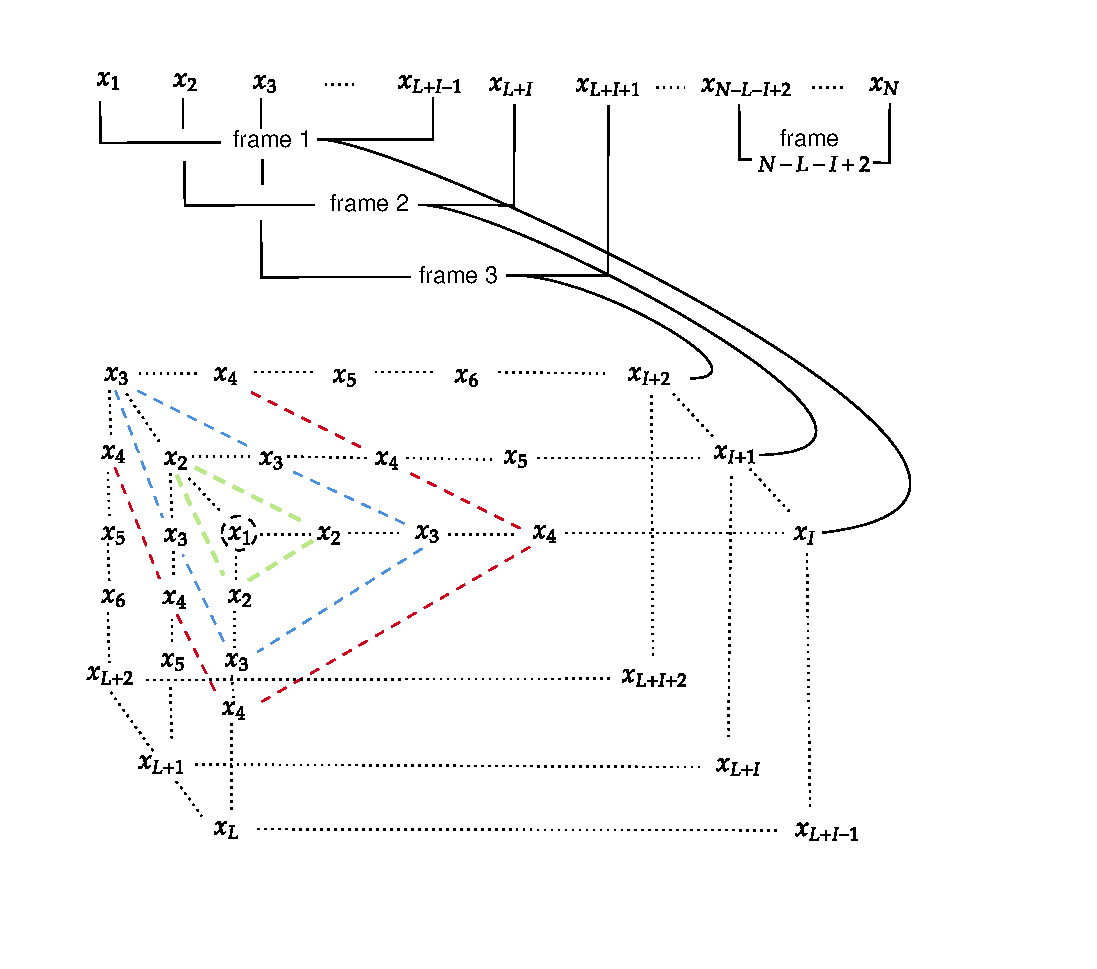
\includegraphics[width=0.8\textwidth, height=0.8\textheight]{img/tensor_injection_diagram}

        $I, L$ --- параметры
    \end{frame}


    \begin{frame}{Разложение и группировка}
        \begin{itemize}
            \item HOSVD траекторного тензора $\calX$ имеет вид
            \[
                \calX = \sum_{i=1}^{I} \sum_{l=1}^{L} \sum_{j=1}^{N-I-L+2} \mathcal{Z}_{i,l,j} \mathbf{U}^{(1)}_{i}
                \circ \mathbf{U}^{(2)}_{l} \circ \mathbf{U}^{(3)}_{j}.
            \]

            \vspace{0.6cm}
            \itemТогда этап группировки в алгоритме HOSVD SSA имеет вид
            \[
                \calX = \sum_{i=1}^{R} \sum_{l=1}^{R} \sum_{j=1}^{R} \mathcal{Z}_{i,l,j} \mathbf{U}^{(1)}_{i}
                \circ \mathbf{U}^{(2)}_{l} \circ \mathbf{U}^{(3)}_{j},
            \]
            $R\leqslant \min(I, L, N - I - L + 2)$ --- параметр алгоритма.
        \end{itemize}
    \end{frame}
    
        \begin{frame}{Ранг в тензорном варианте}
        \begin{itemize}
            \item \bluetext{$n$-ранг тензора:} размерность пространства, порождённого
            векторами вдоль $n$-го измерения.

            \item В отличие от матричного случая, $n$-ранги тензора произвольной размерности могут в общем случае
            не совпадать.
        \end{itemize}

        \begin{statement}
            Пусть временной ряд $\tX$ имеет конечный ранг $r$ в терминах \emph{SSA}\@.
            Тогда для любых значений параметров $I$ и $L$ таких, что
            \[
                r\leqslant\min(I, L, N-I-L+2),
            \]
            все $n$-ранги траекторного тензора $\mathcal{X}$
            этого ряда с параметрами $I$ и $L$ будут равны $r$.
        \end{statement}
    \end{frame}

    \begin{frame}{Численное сравнение}
        Сигнал $s_n = 30\cos(2\pi n/12)$, $n\in \overline{1:71}$.
        Шум гауссовский, белый с $\sigma=5$ и красный с $\delta=\sqrt{5}$,
        $\varphi_1=0.5$ или $\varphi_2 = 0.9$.

        \footnotesize
        \begin{table}[ht]
            \centering
            \caption{RMSE восстановленного с помощью SSA сигнала.}
            \begin{tabular}{r|rrrr}
                \hline
                \backslashbox{вид шума}{$L$} & 12   & 24   & 30            & 36   \\
                \hline
                белый, $\sigma=5$         & 1.82 & 1.42 & \textbf{1.40} & 1.42 \\\hline
                красный, $\varphi=0.5$       & 1.31 & 1.03 & \textbf{1.01} & 1.03 \\\hline
                красный, $\varphi=0.9$       & 1.88 & 1.37 & \textbf{1.34} & 1.36 \\
                \hline
            \end{tabular}
        \end{table}
        \begin{table}[!ht]
            \centering
            \caption{RMSE восстановленного с помощью HOSVD SSA сигнала.}
            \begin{tabular}{r|rrrrrr}
                \hline
                \backslashbox{вид шума}{$I\times L$} & 12$\times$12 & 12$\times$24  & 12$\times$30 & 24$\times$24 & 24$\times$30 & 30$\times$36 \\
                \hline
                белый шум, $\sigma=5$             & 1.64         & 1.53          & 1.57         & 1.66         & 1.62         & \textbf{1.49} \\
                \hline
                красный шум, $\varphi=0.5$           & 1.18         & 1.12          & 1.14         & 1.21         & 1.19         & \textbf{1.08} \\
                \hline
                красный шум, $\varphi=0.9$           & 1.58         & \textbf{1.44} & 1.47         & 1.57         & 1.54         & 1.46          \\
                \hline
            \end{tabular}
        \end{table}
    \end{frame}


    \section{Tensor MSSA}\label{sec:tens_mssa}
    \begin{frame}{MSSA}
        \bluetext{Многомерный временной ряд:}

        $\tX = (\tX^{(1)}, \tX^{(2)}, \dots, \tX^{(p)})^\rmT, \qquad
        \tX^{(i)} = (x_1^{(i)}, x_2^{(i)}, \dots, x_N^{(i)})$.

        \vspace{0.6cm}

        \bluetext{Траекторная матрица этого ряда:}

        $\bfX = [\bfX^{(1)}; \bfX^{(2)}; \dots; \bfX^{(p)}],$

        $\bfX^{(i)}$ --- траекторная матрица $\tX^{(i)}$.

        \vspace{0.3cm}

        Дальнейшие шаги алгоритма (разложение траекторной матрицы и восстановление сигнала) аналогичны стандартному SSA.

        \vspace{0.6cm}

        \begin{itemize}
            \item В случаях, когда ряды $\tX^{(i)}$ имеют похожую структуру, использование MSSA даёт
            лучшие результаты в задаче выделения сигнала, чем применение SSA
            к каждому ряду отдельно.
        \end{itemize}
    \end{frame}

    \begin{frame}{Тензорная модификация MSSA}
        Вместо матрицы $\bfX = [\bfX^{(1)}; \bfX^{(2)}; \dots; \bfX^{(p)}]$

        тензор $\calX:~\calX_{,,i} = \bfX^{(i)}$

        \begin{center}
            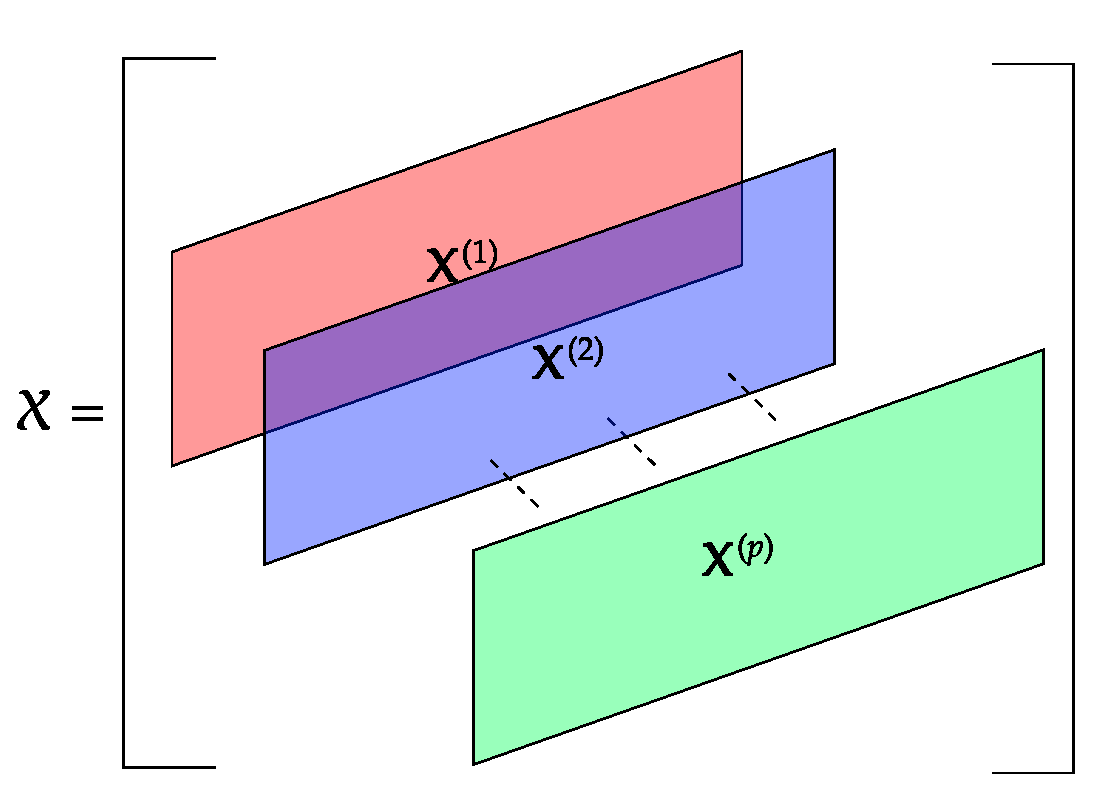
\includegraphics[width=0.8\textwidth, height=0.75\textheight]{img/mssa_injection}
        \end{center}
    \end{frame}

    \begin{frame}{Тензорная модификация MSSA}
        Утверждение, позволяющее перенести понятие ранга ряда на тензорный вариант MSSA.

        \vspace{0.2cm}

        \begin{statement}
            Пусть $\mathbf{A} = [\mathbf{H}_1; \mathbf{H}_2; \ldots; \mathbf{H}_p] \in \mathbb{C}^{L\times Kp}$,
            её SVD имеет вид:
            \[
                \mathbf{A} =\mathbf{U} \mathbf{\Lambda} \mathbf{V},
            \]
            и пусть $\mathcal{A}: \mathcal{A}_{,,i} = \mathbf{H}_i \in \mathbb{C}^{L\times K \times p}$, его HOSVD имеет вид:
            \[
                \mathcal{A}=\mathcal{Z} \times_1 \hat{\mathbf{U}}_1 \times_2 \hat{\mathbf{U}}_2 \times_3 \hat{\mathbf{U}}_3.
            \]

            Тогда существуют такие SVD матрицы $\bfA$ и HOSVD тензора $\calA$,
            что $\bfU = \hat{\bfU}_1$.
        \end{statement}
    \end{frame}

    \begin{frame}{Ранги в тензорном MSSA}
        \begin{itemize}
            \item Если ряд $\tX$ имеет ранг $r$ в терминах SSA, то при $r \leqslant \min(L, K)$ выполнено
            $\operatorname{rank}_1(\calX) = r$.
            \item По симметричности построения, в этих предположениях $\operatorname{rank}_2(\calX) = r$.
            \item Однако ранг третьего измерения приобретает иной смысл.
        \end{itemize}

        В тензорном варианте алгоритма к параметрам $L$ и $R$ \bluetext{добавляется} параметр~$R_3$.

        \vspace{0.5cm}

        \bluetext{Примеры}

        \vspace{0.1cm}

        $x_n^{(m)}=a_m \sin(2\pi n \omega_m + \psi_m),\, m \in \{1,\, 2\},\, n\in \overline{1:N},$

       $a_m\ne 0,\, 0<\omega_m<\frac 1 2,\, 0 \leqslant \psi < 2 \pi$

        \vspace{0.1cm}

        \begin{enumerate}
            \item $\psi_1 = \psi_2,\, \omega_1 = \omega_2 \implies r = r_1 = r_2 = 2,\, r_3 = 1$,
            \item $\psi_1 \ne \psi_2,\, \omega_1 = \omega_2 \implies r = r_1 = r_2 = 2,\, r_3 = 2$,
            \item $\hspace{4em}\, \omega_1 \ne \omega_2 \implies r = r_1 = r_2 = 4,\, r_3 = 2$.
        \end{enumerate}
    \end{frame}

    \begin{frame}{Численные сравнения}
        $x_n^{(m)} = a_m \cos(2\pi n \omega_m + \psi_m),\, n\in\overline{1:71},\, a_1 = 30,\, a_2 = 20$.

        \vspace{0.3cm}

        Шум --- белый гауссовский, с параметром $\sigma=5$, RMSE было сосчитано по 500 реализациям зашумлённого ряда,
        сравнение проводилось на одних и тех же реализациях шума.
    \end{frame}

    \begin{frame}{Численные сравнения}
%        \footnotesize
        \begin{table}[!ht]
            \centering
            \caption{RMSE восстановленных различными методами сигналов для каждого набора параметров сигнала.}
            \def\arraystretch{1.7}
            \resizebox{\columnwidth}{!}{
            \begin{tabular}{r|r|rrrrr}
                \hline
                Условия & \backslashbox{Метод}{$L$}  & 12   & 24   & 36   & 48           & 60   \\ \hline
                \multirow{2}{*}{
                \begin{tabular}{r}
                           $\omega_1 = \omega_2 = \frac 1 {12}$\\
                           $\psi_1 = \psi_2 = 0$\\
                \end{tabular}
                } & MSSA & 1.78 & 1.34 & 1.25 & \textbf{1.20} & 1.41 \\ \cline{2-7}
                  & HOSVD MSSA & 1.35 & \bluetext{\textbf{1.10}} & \bluetext{\textbf{1.10}} & \bluetext{\textbf{1.10}} & 1.35 \\ \hhline{=|=|=====}
                \multirow{2}{*}{
                \begin{tabular}{r}
                    $\omega_1 = \omega_2 = \frac 1 {12}$\\
                    $\psi_1 = 0,\, \psi_2 = \frac \pi  4$\\
                \end{tabular}
                } & MSSA & 1.78 & 1.34 & 1.25 & \textbf{1.20} & 1.41 \\ \cline{2-7}
                  & HOSVD MSSA & 1.41 & \bluetext{\textbf{1.19}} & 1.20 & \bluetext{\textbf{1.19}} & 1.41 \\ \hhline{=|=|=====}
                \multirow{2}{*}{
                \begin{tabular}{r}
                    $\omega_1 = \frac 1 {12},\, \omega_2 = \frac 1 8$\\
                    $\psi_1 = 0,\, \psi_2 = \frac \pi  4$\\
                \end{tabular}
                } & MSSA & 2.63 & 1.94 & 1.74 & \textbf{1.69} & 1.95 \\ \cline{2-7}
                  & HOSVD MSSA & 1.95 & \bluetext{\textbf{1.67}} & 1.69 & \bluetext{\textbf{1.67}} & 1.95 \\ \hline
            \end{tabular}
            }
        \end{table}
    \end{frame}

    \section{Выводы}\label{sec:conclusion}
    \begin{frame}{Выводы}
        \begin{itemize}
            \item HOSVD SSA и HOSVD MSSA являются прямыми обобщениями SSA и MSSA, однако устроены
            существенно сложнее и имеют б\'{о}льшую трудоемкость.
            \vspace{0.2cm}
            \item Оба расширения усложняют алгоритм необходимостью подбора дополнительного параметра.
            \vspace{0.2cm}
            \item HOSVD SSA выделяет сигнал менее точно, чем SSA\@.
            \vspace{0.2cm}
            \item HOSVD MSSA выделяет сигнал точнее, чем MSSA\@.
        \end{itemize}
    \end{frame}
\end{document}
